%
%  $Description: Author guidelines and sample document in LaTeX 2.09$
%
%  $Author: ienne $
%  $Date: 1995/09/15 15:20:59 $
%  $Revision: 1.4 $
%

\documentclass[times,10pt,twocolumn]{article}
\usepackage{depth}
\usepackage{times}
\usepackage{balance}
\usepackage{graphicx}
\usepackage[font=small,labelfont=bf]{caption}

%\documentstyle[times,art10,twocolumn,latex8]{article}

%-------------------------------------------------------------------------
% take the % away on next line to produce the final camera-ready version
\pagestyle{empty}

%-------------------------------------------------------------------------
\begin{document}

\title{Estimating Surface Orientations Based on Monocular Image Queues}

\author{Alexander Norton\\
\emph{Computer Science Department,}\\
\emph{Colorado State University}\\
\emph{norton@cs.colostate.edu}\\
}

\maketitle
\thispagestyle{empty}

\begin{abstract}
Abstract - Recovering the 3 dimensional structure of a scene from a single 2
dimensional video stream is a task that humans have very little trouble with.
However, when computers attempt the same process, the products are either very
simple, or very prone to error. We present a algorithm that does a simple image
segmentation based with the goal of finding the vertical surface orientations.
Based upon the relative orientations of the different regions of the image, the
relative depth of objects of interest within the video can then be estimated.
We provide a quantitative analysis of the algorithm of a set of monocular
outdoor images and a qualitative analysis on video data.
\end{abstract}

%-------------------------------------------------------------------------
\Section{Introduction}

Reconstruction of the 3 dimensional scene geometry is an important step in
understanding a scene and interpreting the interactions between the objects
within that scene. Understanding the relative depth of two distinct object can
help inform the relationship between them. For example, one could infer if the
two objects would be able to touch based upon not only how close they are in
the pixel space, but also how close they fall in relative depth. There has been
work on create a full reconstruction in the form of a pop-up model from a
single monocular image~\cite{Hoiem-05, Hoiem-08, Sexana}. Gupta, Efros and
Hebert~\cite{Gupta} improved upon this by creating volumetric versions by
trying to recreate the blocks in the monocular image using a 3 dimensional
model. Other forms of scene reconstruction depend upon used know motion of the
camera, stereo vision or other similar techniques to find the geometry.

\begin{figure}[t]
  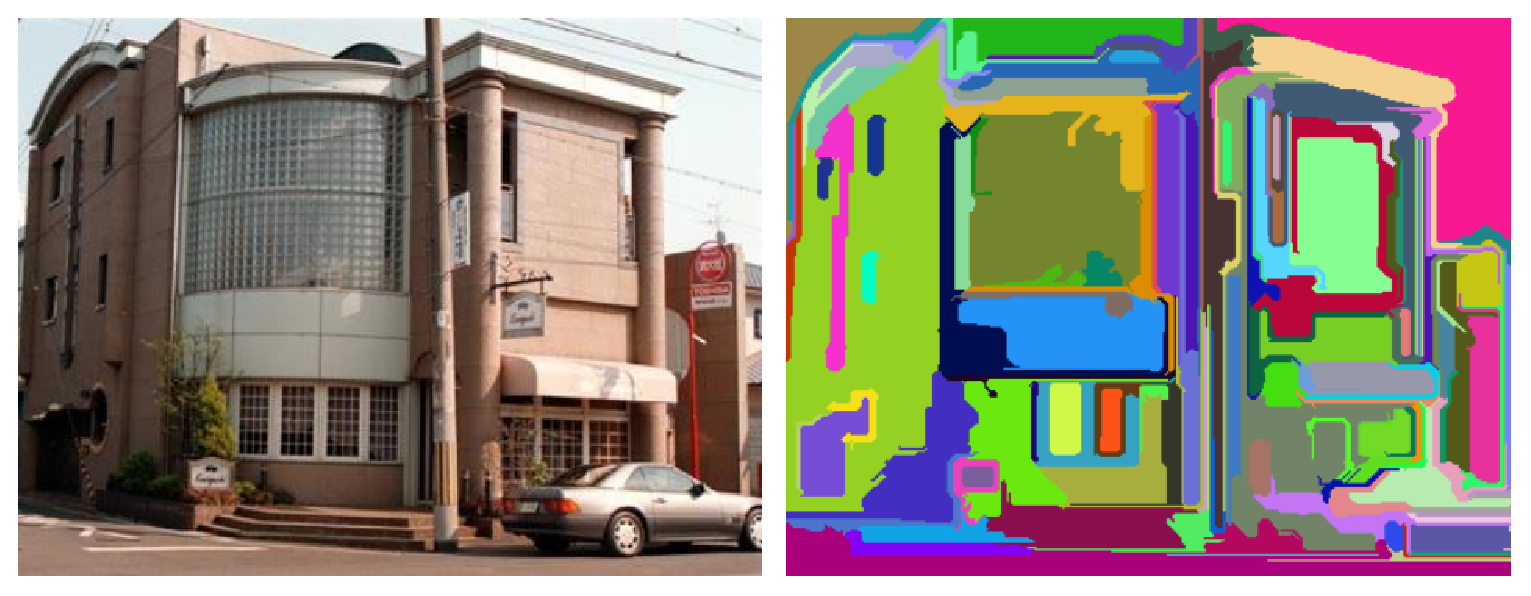
\includegraphics[keepaspectratio=true, width=\linewidth]{segment.eps}
  \caption{A monocular image with the over-segmentation produced by
           Felzenszwalb et al.~\cite{Felzen}. These segments are referred to as
           super pixels.}
  \label{fig:superpixel}
\end{figure}

We propose a algorithm that combines these two efforts. It attempts to
reconstruct the scene geometry from a monocular video instead of a monocular
image. This allows the algorithm to incorporate temporal information into the
surface estimations. However, structure from motion or similar techniques
cannot be applied to the video since there is no information about the camera
or defined camera locations. As a result, the algorithm relies upon the methods
developed by Hoiem et al.~\cite{Hoiem-05} and Sexana et al.~\cite{Sexana} to
find the vertical surface orientations. From this the relative depth of
different regions of the image can be estimated to provide object information.
The goal is to create a depth segmentation of the image.

The algorithm uses supervised learning to create a classifier for image
regions. The algorithm will start with an over-segmentation of the image to
produce super pixels. Super pixels are simply image regions that statistical
information can gathered for. The statistical information is used as input for
the learned classifier which is used to decide the surface orientations. From
the surface orientations we can gather depth information by simply using where
the vertical surfaces intersect the horizontal surface defined by the ground
plane.

%-------------------------------------------------------------------------
\Section{Super Pixels}

\begin{figure*}[t]
  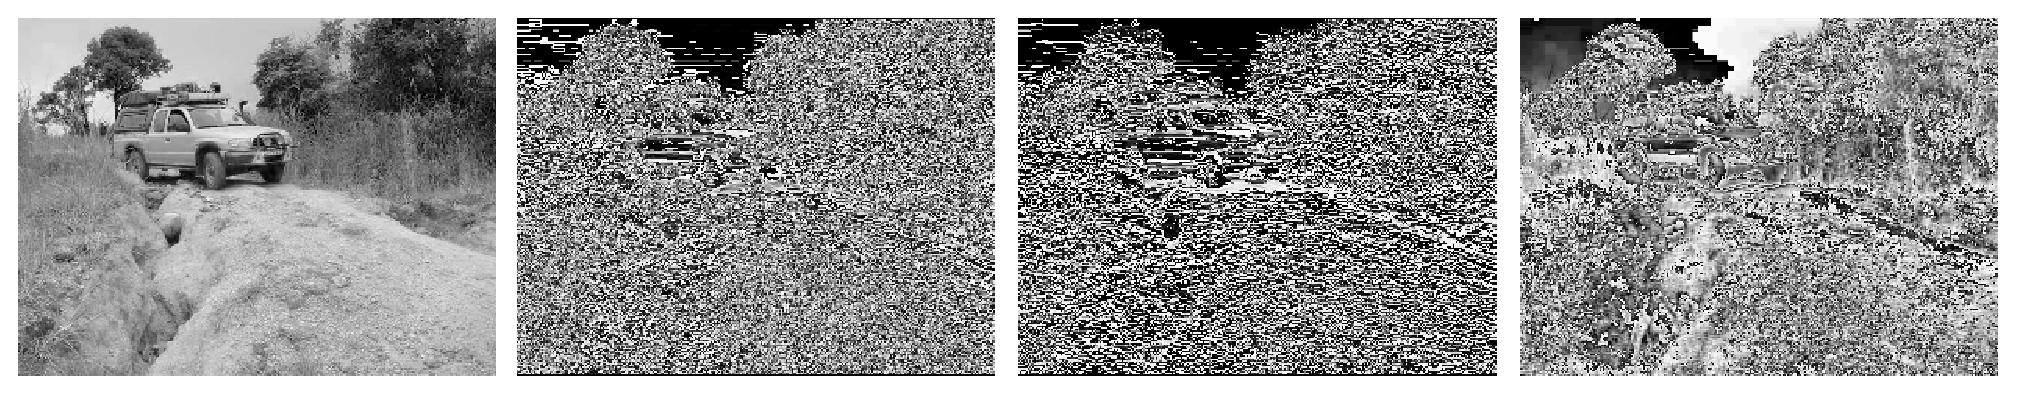
\includegraphics[keepaspectratio=true, width=\textwidth]{Laws.eps}
  \caption{One color channel of a source image with the Law's mask
           convolutions. The average response from these masks is used
           as one of the features for the classifier.}
  \label{fig:lawsconv}
\end{figure*}

The first step in finding a usable depth segmentation is to perform an
over-segmentation of the image. An example of the over-segmentation can be seen
in Figure~\ref{fig:superpixel}. These super pixels will be used as the units
of surface. We will construct the surfaces out of the individual super pixels
and the borders between surfaces will be assumed to fall on the boundaries
between super pixel. As a result of this, the only requirement of the
over-segmentation is that there is no single super pixel that spans two real
world surfaces within the image. If a super pixel does fall on two different
real world surfaces, then it would have multiple orientation and automatically
cause the depth segmentation to be invalid. The algorithm uses the segmenation
algorithm described by Felzenszwalb et al.~\cite{Felzen} to produce the super
pixel image. Any segmentation algorithm could be used in instead as long as it
doesn't produces any segments that contain two distinct real world surfaces.

For each super pixel in the image a set of statistics are calculated. The major
distinguishing factors between horizontal and vertical surfaces are the
textures and line orientations on the surface. As a result, the texture is
calculated as the response the a set of 3x3 Law's masks for the different color
channels of the image. The Law's masks are created using the three vectors
[1, 2, 1], [1, 0, -1], and [1, -1, 1]. These vectors are multiplied to get
9 3x3 masks that are convolved with the color channel. This produces a total of
27 responses from the Law's masks. A source image and some example responses
for the Law's masks can be seen in Figure~\ref{fig:lawsconv}. A histogram of
gradient orientations is calculated for each super pixel as well. 18 buckets
are used for the histogram of gradients, and each color channel uses a
different histogram. This gives a total of 54 buckets from gradient histograms.
This gives an 81 dimensional space that is used to represent the super pixel in
the learned classifier.

%-------------------------------------------------------------------------
\Section{Learned Classifier}

\begin{figure*}[t]
  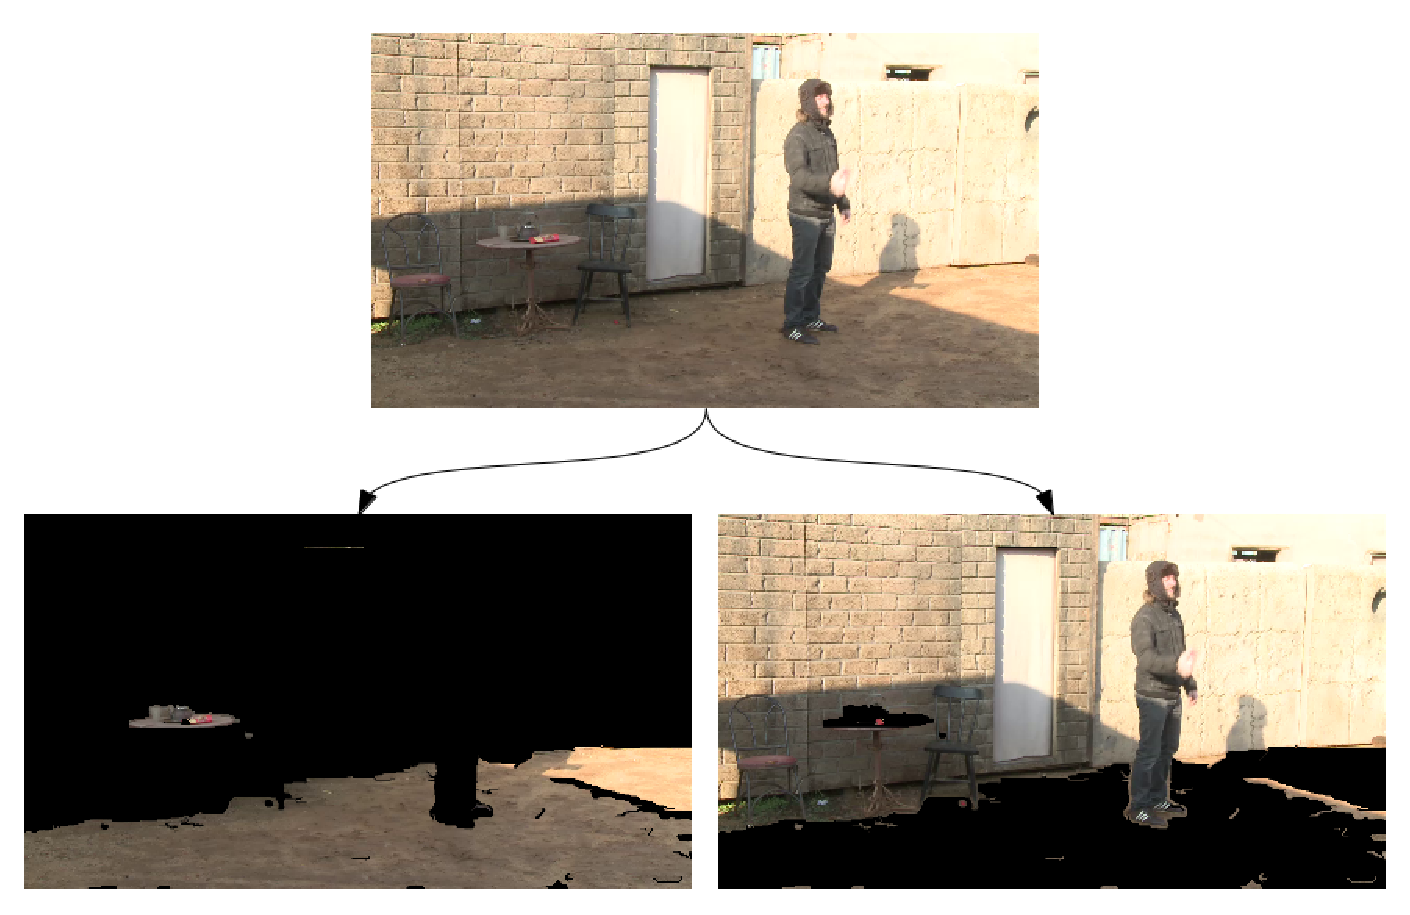
\includegraphics[keepaspectratio=true, width=\textwidth]{split.eps}
  \caption{The output of the classifier. Image regions of the source image
           (the top image) are input into the classifier. The super pixels
           that the classifier decided were horizontal are on the left. The
           vertical are on the right. }
  \label{fig:spliting}
\end{figure*}

\begin{figure*}[t]
  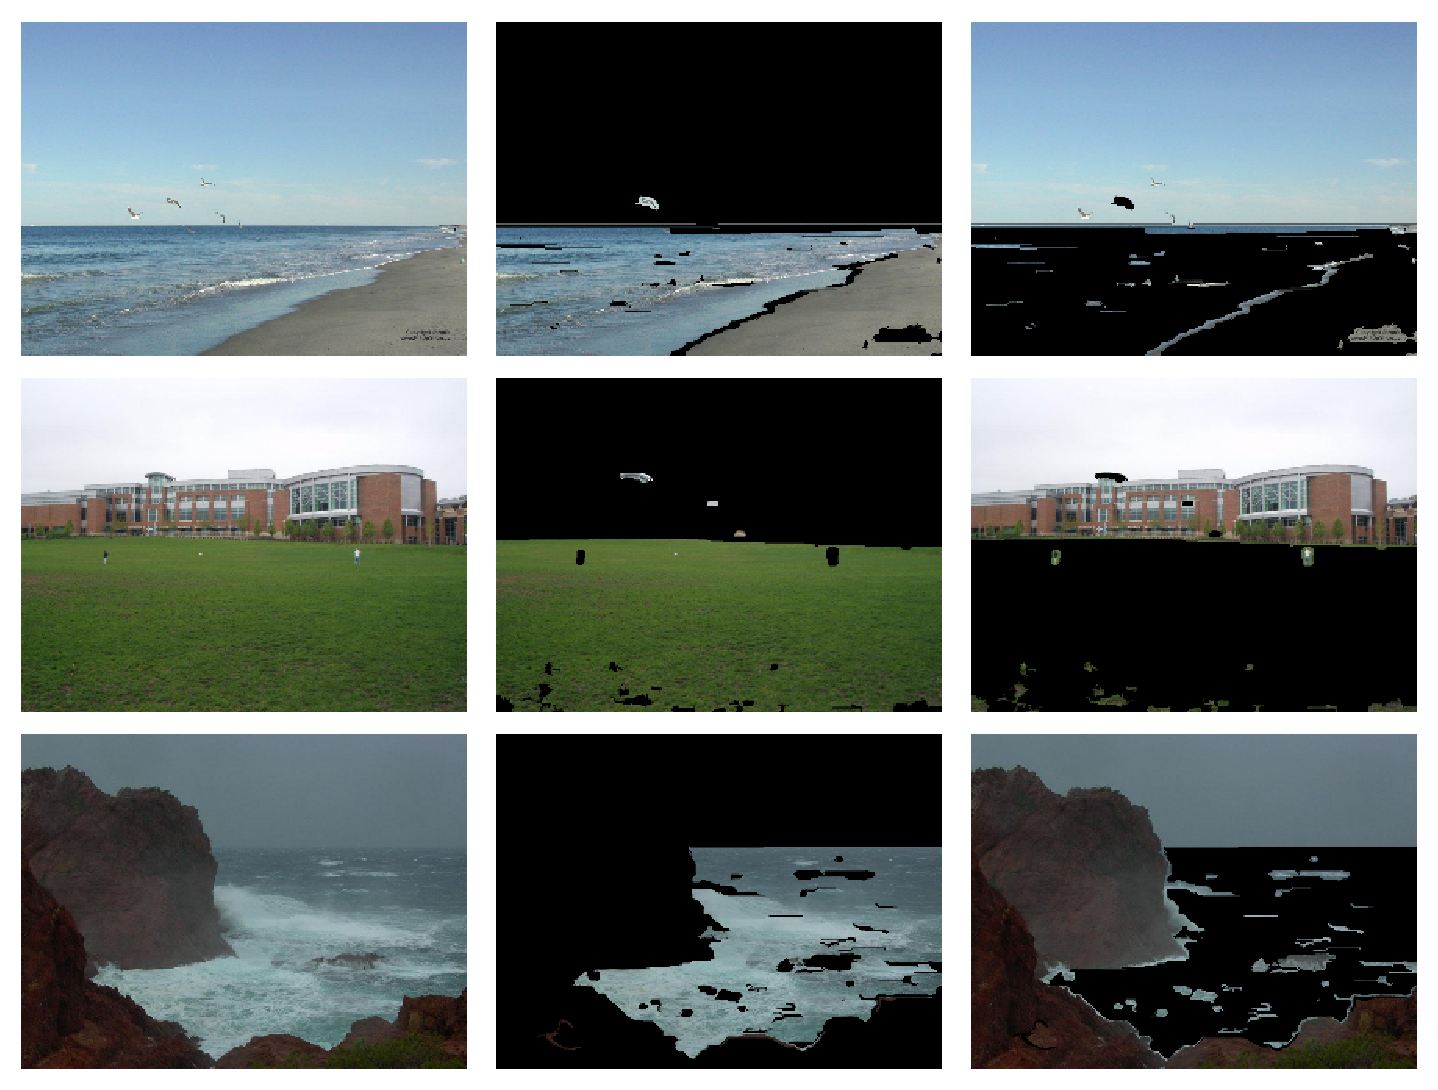
\includegraphics[keepaspectratio=true, width=\textwidth]{Good.eps}
  \caption{ Examples or correct segmented images. The first column is the
            original source image. The middle column is the horizontal segment
            of the image. The right column is the vertical segment of the image}
  \label{fig:correct}
\end{figure*}

The collection of features used for each super pixel is fed into a learning
classifier that will inform the algorithm about the orientations of the super
pixels. Both grouping the super pixels together into larger image regions and
testing super pixels completely independently was tried. Two different learned
classifiers were used. The discrete form of Adaboost and a simple k-nearest
classifiers were both tested and the results compared. These were used because
of the simplicity involved in using them correctly.

Both individual super pixels and small image regions were used as input for the
classifier. These were tested individually for the training and testing phases.
The rational behind testing image region is that the orientation can be
informed by what lies around the super pixel. For example, take the case of a
brick wall where the boundaries between the super pixels would fall at the edge
of each brick. If we include adjacent super pixels in the calculation of the
score for the relevant super pixel, then we can include more of the texture of
the brick wall. We are pulling more information into the surface estimations in
the hopes that we will get a better response.

The classifier was tested on 17 labeled training images. These images were
labeled by hand with the possibilities of vertical, horizontal, sky or other.
For the classifier, the category of sky was changed for vertical. There is
reason to find sky separately from other images categories since it can be
interpreted as having an infinite depth. However, to simplify the classifier,
this category was treated as vertical.

Once an image has been over-segmented, each super pixel is used as input into
the classifier. The results of the classifier are then used to directly label
the image as either vertical or horizontal. The image is split into these two
separate segments as in Figure~\ref{fig:spliting}.

%-------------------------------------------------------------------------
\Section{Results}

The algorithm was tested on a set of 300 images of outdoor scenes. Of these
images, the number of super pixel correctly labels was used to determine if the
algorithm adequately labeled that image. The k-nearest classifier was not
rigorously tested as it was simply a proof of concept. However, based upon
some qualitative analysis, the k-nearest classifier performed much better than
expected. It would correctly label enough super pixels to identify the vertical
and horizontal images.

For the Adaboost classifier, both individual super pixels and image regions
were tested. When building the image regions for training, the region for a
particular super pixel included all adjacent super pixels that were of the same
class. This would mean that the training didn't include a mixing of classes and
would avoid confusing the classifier. For testing, the region simply consisted
of all adjacent super pixels. As we do not know what class two super pixel
belong to during testing, we assume that the most common case (i.e. they do
belong to the same surface) is the correct case.

For individual super pixels with the Adaboost classifier, the algorithm
correctly estimated the horizontal and vertical surfaces for 145 of the 300
test images. For regions of super pixels with the Adaboost classifier, the
algorithm got 104 image correctly estimated. This is a accuracy of \%48.3 for
individual super pixels and \%34.6 for the super pixels that were grouped into
regions. It is important to note that while there was significant overlap
between the sets of images that both correctly estimated, there were several
notable exceptions that did not appear in both sets of correctly guessed
images.

Qualitatively, on the limited number of videos of outdoor scenes that the
algorithm has been run on, it has done well segmenting the image. Interestingly
the results of the algorithm from one frame to the next can change drastically.
This would indicate that small changes to the underlying pixels can result in
a very different response from classifier. This may be due to a drastic change
to the segmentation.

%-------------------------------------------------------------------------
\Section{Conclusion}

We set the goal of creating an algorithm that could perform an image
segmentation that would allow for estimations of horizontal and vertical
surface orientation estimation. We have taken important steps towards
accomplishing this goal. Given a relatively simple outdoor scene, we can
correctly determine what surfaces within the image are horizontal and which are
vertical. From the successful image segmentations we have shown that simple
texture and gradient orientations contain enough information to estimate the 3
dimensional orientation of the underlying surface.


However, we have also shown that something that should logically improve the 
surface orientation estimation, namely taking the neighbors of a super pixel
into account, actually decreased the quality of the vertical surface
orientation estimation. Hoiem et al.~\cite{Hoiem-05} use a learning pairing
function to guess when two super pixels belong to the same class. Also the set
of images correctly labeled by region classifier is not a subset of the images
correctly labeled by the individual classifier. These would indicate that
the performance of the algorithm could possibly be improved by not necessarily
including every neighbor when creating the region. Something similar to the
learned pairing function used in Hoiem et al.~\cite{Hoiem-05} should be
explored.

%-------------------------------------------------------------------------
\bibliographystyle{depth}
\bibliography{depth}

\end{document}

